\chapter{Design}

As an instrument, space purpose, we were aimed to create a lidar with the smallest possible sizes, small consumption and small mass.
The concept we are developing (MEMS-based lidar with small FOV), basically, is a unique technology that allows achive all our goals.

Today most of the modern LiDARs are based on motor scanning, however MEMS mirrors are commonly used in LiDARs too (Fig. \ref{fig:concept_1}).

\begin{figure}[h]
\center{\includegraphics[width=1\linewidth]{concept_1}} 
\caption{A typical schematic of MEMS mirror-based LiDAR. Laser beam is steered by the MEMS mirror. On the contrary, the detector looks everywhere, and it has a large FOV and consequently low SNR.}
\label{fig:concept_1} 
\end{figure}

The advantage of using MEMS mirror instead of a motor is the significant decrease of LiDAR’s size and mass in comparison. However, there are disadvantages like a small FOV (order of 20$^\circ$ instead of 360$^\circ$ in case of rotating) and a small receiver aperture, which is limited by the size
of the MEMS mirror.


The number of background photons is proportional to the square of the detector’s FoV size, therefore when the FoV size is decreased from the typical 20-30 degree to 0.1 degree,
the background decreases $~10^5$ times.
As a result of which a new approach was developed: detector's FOV is steering by MEMS mirror together with a laser beam, that enables to reach large distance sensitivity by dramasticaly increasing SNR ignores all of the background (Fig. \ref{fig:concept_2}).

The peak laser photon rate and solar photon rate, $[\#s^{-1}]$ are calculated as\footnote{
Where $P_{laser}$ and $\nu$ is peak power and frequency of the laser corresondingly, $r_{lens}$ and $\theta$ are respectively the radius and the FOV of the detector, $d_{range}$ is distance from target to detector, while $\eta$ is reflectance of object. $PD_{sun}$ is the solar power density calculated by integrating the spectral power density between $\lambda - \delta\lambda$ and $\lambda + \delta\lambda$ with $\delta\lambda$ being half the bandpass of the optical filter on the detector.
}
:
\begin{equation}\label{eq:peak_power}
\Phi_{laser} = P_{laser} \cdot \eta \cdot \frac{1}{2\pi d_{range}^2} \cdot \pi r_{lens}^2 \cdot \frac{1}{h\nu}
\end{equation}
\vspace{-5mm}
\begin{equation}\label{eq:sun_noise}
\Phi_{solar} = PD_{sun}(\lambda \pm \delta \lambda) \cdot \pi (r_{lens}+d_{range} \cdot tan\frac{\theta}{2})^2 \cdot \eta \cdot \frac{1}{2\pi d_{range}^2} \cdot \pi r_{lens}^2 \cdot \frac{1}{h\nu}
\end{equation}

Thus with a combination of a narrow band-pass optical filter and quick enough electronics readouts, the background drops as low as 0-1 photon per sampling time. It becomes possible to distinguish a signal that consists only of 2-3 photons.
In order to match FOVs both SiPM and laser beam two diffrent approaches can be used.
Since the diode has a polarization (10:1), the natural way is to use a polarizer, in this case laser power output is ~90\% and received ~50\%, finally the efficiency is about 45\%.
Another way is using left part of the MEMS mirror for transimtting laser beam and right part for receiving. In this case efficiency will be around 25\%.
Currently, second approach was done, since in case of beam-splitter, to many stray-light appears that make SiPM blind for some time. But it can be improved by changing readout electronics later.


\begin{figure}[h]
\center{\includegraphics[width=1\linewidth]{concept_2}} 
\caption{
Schematic of MEMS pinhole LiDAR. Both laser beam and detector FoV are steering by the MEMS mirror, they have all time same FOV, thereby ignoring background. This concept allows a much higher SNR and consequently much higher distance range.
}
\label{fig:concept_2} 
\end{figure}


A further advantage of our LiDAR that we made is silicon photomultiplier (SiPM)
sensor. The Silicon Photomultiplier (SiPM) is a single-photon sensitive sensor that has performance characteristics comparable to a conventional ICCD/PMT/APD. with the practical advantages of a solid-state sensor.
By combining a narrow FOV of the detector collimator and SiPM sensor, we increase LiDAR sensitivity several hundred times over. Therefore, the resulting LiDAR does not require huge aperture lenses, and it may be implemented as one or two orders smaller in size than other existing LiDARs without the loss any of its parameters, such as the distance measurement range.

The TOF principe is illustrated in Figure \ref{fig:algo}. In the direct ToF technique, a laser pulse is directed
at the target. The target diffuses and reflects the laser photons and some of the photons are reflected back towards
the sensor. The sensor converts the detected laser photons (and some detected photons due to noise) to electrical
signals that are then timestamped by the timing electronics - TDC (Time to Digital Converter).
Whence the distance to the target can be calculated as \footnote{Here, c is speed of light}:

\begin{equation}\label{eq:peak_power}
D = \frac{c \cdot \Delta t}{2}
\end{equation}

The sensor must discriminate returned laser photons from the noise (ambient light). The timestamp is captured when the threshold is exceeded.
This is known as a single-shot measurement.
The signal to noise ratio can be dramatically improved by using average, when the data from many singleshot measurements are combined
to produce a ranging measurement from which the timing of the detected laser pulses can be extracted with high precision and accuracy.

\begin{figure}[h]
\center{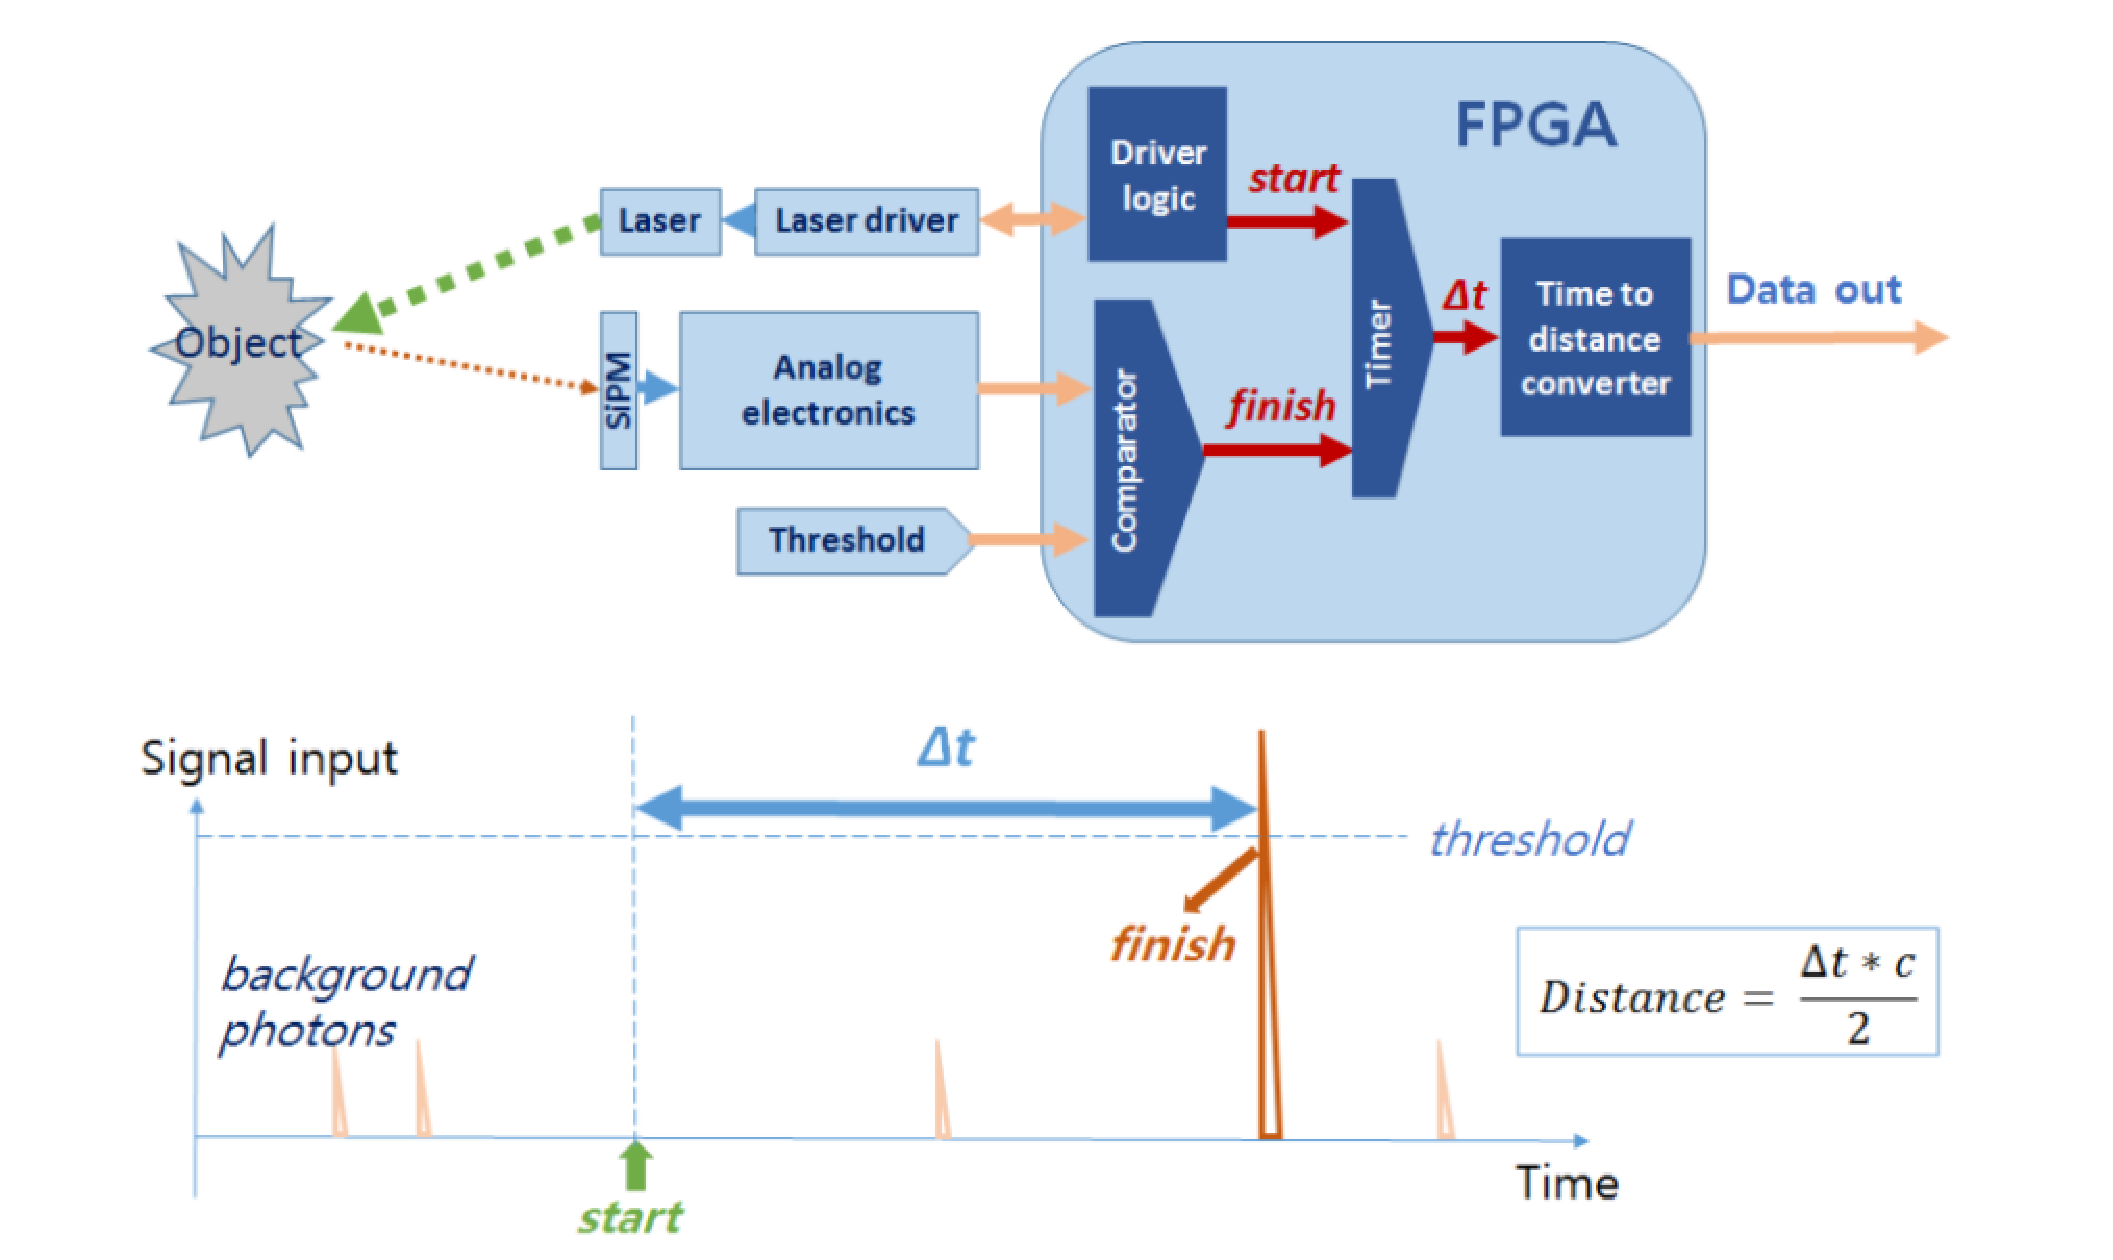
\includegraphics[width=1\linewidth]{algo}} 
\caption{
Signal processing outline and distance measurement by TOF method.}
\label{fig:algo} 
\end{figure}


Our lidar system consist of the following components:
\begin{enumerate}
\itemsep-0.5em 
\item  \textbf{Laser module:} A pulsed laser with collimation optics and driver circuit.
\item \textbf{SiPM module:} SiPM sensor with detection optics (include bandpass filter) and discriminator circuit.
\item  \textbf{MEMS module:} MEMS mirror + driver circuit.
\item  TDC and data processing electronics CPU/FPGA-based, and communications interface.
\item  PC based software.
\end{enumerate}
The chapter 3 focuses on system design of first three of these items.

Short description of the system:
The lidar uses a 905 nm laser diode with a pulse width of 10ns and a peak laser power of up to 90 W at repetition rate up to 12 kHz.
The laser output signal is collimated by a lens with a divergence of 0.1$^\circ$ x 2.5$^\circ$.
At the receiver the reflected signal is focused on the sensor using a 4.5 mm focal length collection lens with an aperture of 3.7 mm diameter.
The sensor angle of view is 2.8$^\circ$.
The signal is also filtered by an optical bandpass filter with a FWHM of 10nm.
The detection signal chain consists of a SensL MicroRB-10035 SiPM, a gain stage and a high-speed
comparator, which performs leading edge discrimination, and pulse generator circuit.
The mems have diameter of 3.6 mm and the scanning FOV of 25$^\circ$ x 13$^\circ$ with scanning speed of 12 FPS for 8 lines. 
The resulting pulses are timestamped using a standalone TDC and data acquisition system.
The acquired data is transferred to PC software via a high speed USB link.


